\chapter{Teorie}
\label{2-teorie}

Před vynalezením malých mikroprocesorů pro řízení letu byl upřednostňován klasicický způsob letu (letadla, vrtulníky) před drony. Po vynalezení těchto mikroprocesorů byl započat vývoj dronů.\\
Motory s vrtulemi fungují jako ventilátory, které ženou vzduch pod sebe. Bohužel rozložení hmotnosti drona a drobné rozdíly v motorech, zapříčiní různé tahy na jednotlivých motorech. Díky ovládání motorů podle mikroprocesorů, dokážeme vliv různých tahů vyrovnat a dron může létat.\\
Let drona je způsoben snížením výkonu na motory ve směru letu a zvýšením výkonu na motory v opačném směru letu.
%https://www.wired.com/2017/05/the-physics-of-drones/
\begin{figure}[h]
	\centering
	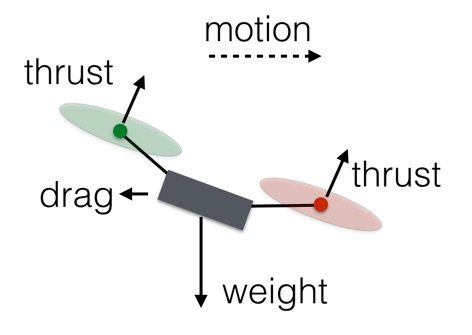
\includegraphics[width=5cm]{pictures/dronfly.jpg}
	\caption{Let určitým směrem}
\end{figure}
 Rotace drona je uskutečněna zvýšením výkonu na různých typech vrtulí (CW a CCW orientace). Zvýšením výkonu na motorech s vrtulemi s orientací CW se dron otáčí po směru hodinových ručiček, s orientací CCW proti směru hodinových ručiček.\\
\begin{figure}[h]
	\centering
	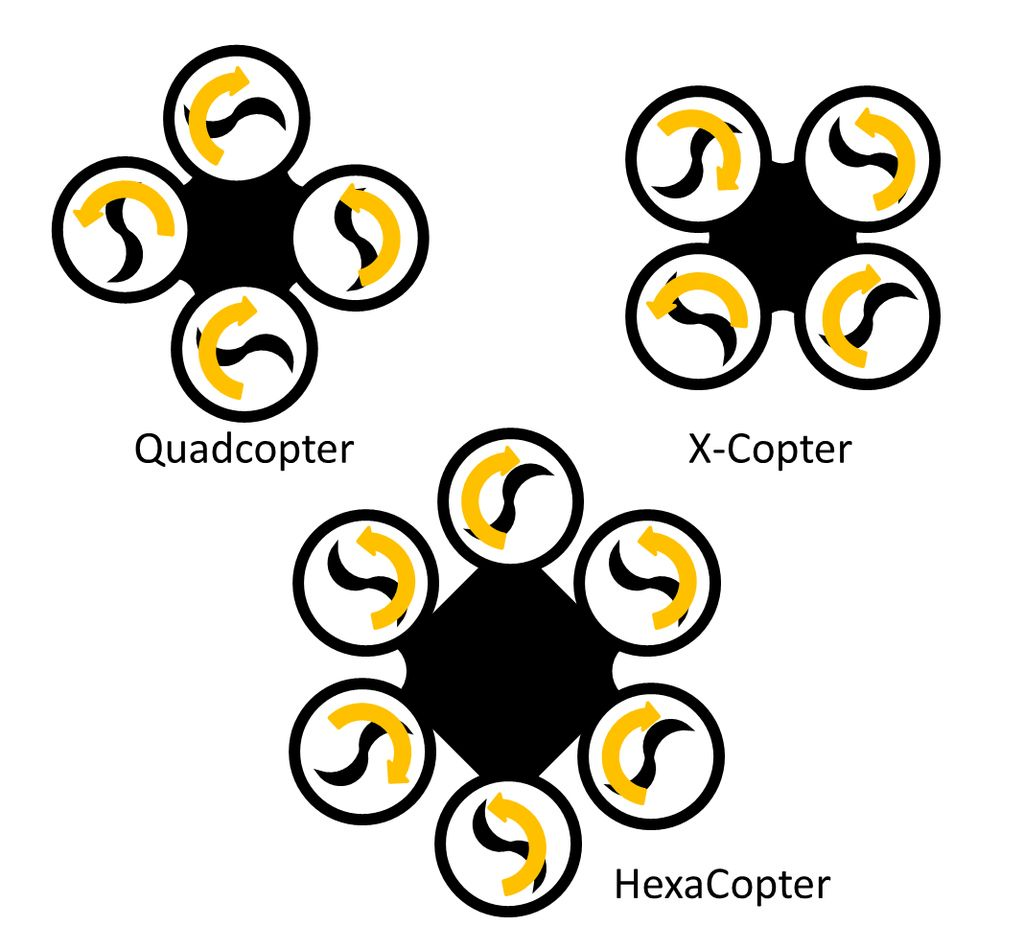
\includegraphics[width=10cm]{pictures/dronrot.png}
	\caption{Přehled vtrulí se CW a CCW orientací}
\end{figure} 
%Source: https://www.instructables.com/id/Design-Build-and-Improve-a-Quadcopter/
Důležitou roly při letu drona hraje IMU jednoka, která určuje úhly náklonů. Roll je úhel rotace kolem osy X, pitch je úhel rotace kolem osy Y a yaw je úhel rotace kolem osy Z. Souřadný systém má střed v težíšti letadla. Osa X směřuje do směru letu, osa Y je na ni kolmá a osa Z je totožná s tížnicí.\\
Řízení drona probíhá přes jmenované úhly pitch, roll a yaw. Uživatel zadává chtěné úhly a mikrokprocesor podle IMU dané úhly nastavuje. Nastavení úhlu vzniká přes ovládání jednotlivých motorů.\\

%https://devusa.djicdn.com/images/flightController-concepts/altitude-7e757661b6.png
\begin{figure}[h]
	\centering
	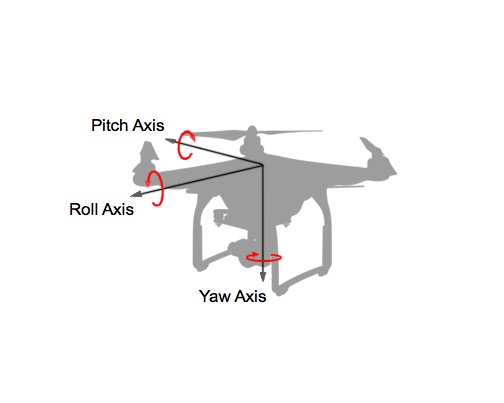
\includegraphics[width=6cm]{pictures/rotangle.png}
	\caption{Úhly rotace/náklonů}
\end{figure} 
